eKwip consists of several components that all work together to collect data about the position and motion of the knee and leg, send the data over a wireless network link to a server, and analyze the data in order to display an image of the knee and collect comprehensive data regarding the motion of the knee.

The process begins in the IMU sensors, which use accelerometers and gyroscopes to measure the absolute orientation, acceleration, and rate of change of acceleration. This data is passed to the microcontroller, which packetizes the data and sends it to the wireless module. The Wifly then transmits the data packets over the wireless network to the server.

The server receives the data packets and parses the data. It then computes the position and movement of the knee in order to display the image of the leg in the graphical user interface and record the position and motion data in a file on the server, which can be used for graphing and further analysis.

Figure~\ref{fig:block_diagram} shows a block diagram modelling the eKwip system.

\begin{figure}[h]
  \begin{center}
    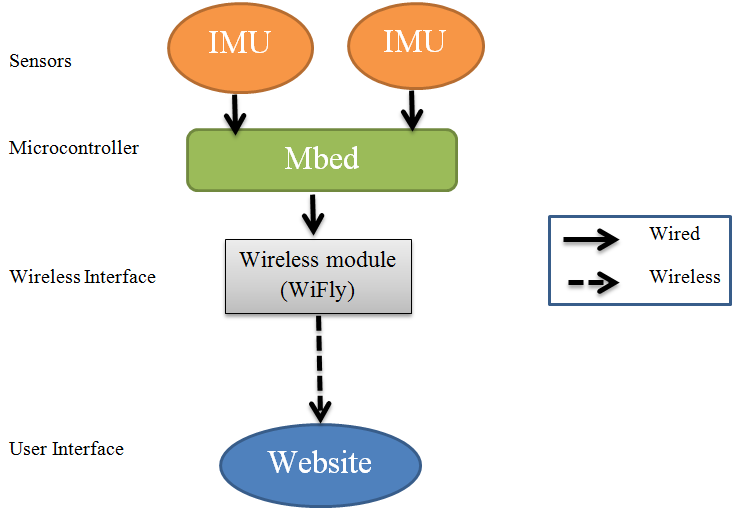
\includegraphics[width=3in]{images/block_diagram.PNG}
  \end{center}
  \caption{Block diagram of eKwip system}
  \label{fig:block_diagram}
\end{figure}

\subsection {Wrap}
eKwip is a spandex wrap that fits around the leg, above and below the knee. A wrap of this type was chosen because it's relatively small, unobtrusive, and stays close to the skin, which is important for correctly measuring the movement of the knee itself, instead of the movement of the wrap. The wrap was designed to be unobtrusive in order to encourage athletes to wear it more often. Unlike current mechanical braces on the market, eKwip does not hinder the movement of the knee, which makes eKwip much more attractive to athletes.

\subsection {Microcontroller}
The microcontroller is responsible for reading data from the sensors and sending the data over the network link. A microcontroller was chosen based on storage capacity, clock speed, ease of use, and the ability to multitask. These are important because a fast processor will allow the reading of data at a high frequency, a decent amount of storage will facilitate the storage of the code libraries in use and to give some initial storage for the data, and the ability to multitask will enable the reading of data and send it over a network link simultaneously. Given all these considerations, the mBed LPC1768 "!!! PLEASE CITE" was selected as an ideal microcontroller for this project.

The mBed is ideal for this project because of its small size and impressive performance. Perhaps most importantly, the mBed has the ability to interface with many different modules at the same time, as it includes three UART serial ports, two SPI ports, two I2C ports, a USB port, a CAN port, and an ethernet port, among other GPIO pins. The mBed contains a powerful 96 MHz ARM Cortex-M3 processor. These features come together to allow several sensors and communication devices to be connected to the mBed at one time.

\subsection {Sensors}
In addition to the microcontroller, eKwip also requires sensors to collect information from the wearer's knee. A set of two inertial measurement units, or IMUs, were selected for this purpose. Two IMUs are required, one on the upper leg and one on the lower leg, so the relative angles of the knee can be measured in order to give an accurate model of the leg. A small IMU that is able to send data very quickly and communicates via UART serial is utilized by eKwip. This allows easy mounting of the IMUs, fast data reading, and easy interface with the mBed. In accordance with all of these considerations, the Pololu UM6-LT "!!! PLEASE CITE" was chosen as the best IMU for this application. The UM6-LT is approximately the size of a quarter, and can measure absolute angles, rate of change of the angles, and acceleration.

An mBed library for the sensors was initially used in order to set up the IMUs and get initial data readings. However, once performance became a concern, it was clear that the library would not give the speed required for the prediction of ACL injuries. The UM6-LT offers two operating modes, broadcast and query. The library used query mode, which involves sending a query to the IMU and waiting for a response. This was the limitation in the speed, so a new library was implemented, which utilizes the UM6-LT's broadcast mode. This allows much faster reading, on the order of 3$\mu$s per data point, as opposed to the previous read time of 30$\mu$s.
